\documentclass{article}
\usepackage[latin1]{inputenc}
\usepackage[spanish]{babel}
\usepackage{amsmath}
\usepackage{amsfonts}
\usepackage{amssymb}
\usepackage{multirow}
\usepackage{graphicx}
%\usepackage{fullpage}
\usepackage[small]{caption}
\usepackage{float}

\renewcommand{\topfraction}{0.9}
\renewcommand{\bottomfraction}{0.8}

\title{Sistemas de Inteligencia Artificial}
\author{Franco Arolfo \and Jorge Mozzino \and Francisco Pagliaricci}


\begin{document}



\begin{titlepage}

\maketitle
\thispagestyle{empty}
\vspace{5cm}
\centerline{\textbf{\LARGE{M\'etodos de b\'usqueda no informados e informados}}}
\vspace{1.24cm}
%\centerline{\textbf{\large{Comisi\'on S}}}
\vspace{3.75cm}
\end{titlepage}


\newpage

\section{Objetivo}
Se propone con este trabajo implementar un Sistema de Producci\'on que ser\'a utilizado para resolver el problema 'Fill Zone'.
A partir de un motor de inferencia programado en Java, se realizaron las respectivas modificaciones para que pudiera trabajar con estrategias de b\'usqueda no informadas (depth first, breadth first y profundizaci\'on iterativa) e informadas (Greedy Search y A*).

\section{Descripci\'on del juego: 'Fill Zone'}
Se le brinda al jugador una grilla de NxN celdas, donde cada celda esta pintada con un color. As\'i mismo, la cantidad de colores a utilizar esta predefinida, en nuestro caso usaremos 6.
Al inicio del juego, dicha grilla cuenta con sus celdas dispersas en forma aleatoria (ver figura \ref{inicial}).

El objetivo del juego es que el tablero finalice con todas sus celdas del mismo color. Para ello, el jugador debe ir cubriendo el tablero de la siguiente manera: por cada turno, debe elegir uno de entre todos los colores disponibles y se pintara a todas las celdas del mismo color que la celda del margen superior izquierdo que sean adyacentes a ella.
Es requerimiento adem\'as que el jugador complete el tablero con un numero m\'aximo de turnos.

Por ejemplo, supongamos que se comienza con el tablero de la figura \ref{inicial}. Eligiendo el color verde en el pr\'oximo turno, se obtendr\'ia el tablero presentado en la figura \ref{regla}.


\section{Desarrollo del proyecto}

\subsection{Preliminares}
Decidimos reutilizar el motor de b\'usqueda desarrollado en Java propuesto por la c\'atedra, modificando lo necesario para nuestro problema.

Las modificaciones realizadas consistieron en generar subclases que implementen los m\'etodos getNode() y setNode(). Dichos m\'etodos var\'ian seg\'un si es un algoritmo no informado o informado, y entre los informados, en donde qu\'e lugar de la cola se sit\'uan los nodos que se visitan.

\subsection{Modelado del problema}
Presentaremos a continuaci\'on nuestro modelo del problema 'Fill Zone':

\emph{Estado:} Modelaremos un estado como un 'board', que consta de una matriz de enteros, y otro entero 'movesLeft', que indica la cantidad de movimientos que el jugador esta permitido a realizar.
En el 'board' decidimos modelar cada color como un entero.

\emph{Estado inicial:} Consta de un 'board' genreado de manera aleatoria, con el 'movesLeft' inicializado con la cantidad de movimientos que se pueden hacer.

\emph{Reglas:} Presentamos las reglas que definimos para el juego:
\begin{enumerate}
	\item El jugador elige color Verde.
	\item El jugador elige color Azul.
	\item El jugador elige color Magenta.
	\item El jugador elige color Blanco.
	\item El jugador elige color Amarillo.
	\item El jugador elige color Rojo.
\end{enumerate}

En todos los casos, el tablero cambia seg\'un lo ya explicado.

\emph{Funci\'on de costos:} Cada regla consume 1 movimiento. De esa forma, teniendo en cuenta que la funci\'on heur\'istica busca estimar la cantidad de movimientos faltantes para resolver el tablero, es l\'ogico que la funci\'on de costo devuelva 1 para todas las reglas.

\emph{Test objetivo:} Un estado es final si todas sus celdas son del mismo color y a\'un quedan movientos por ejecutar, o es el \'ultimo permitido ('movesLeft' >= 0).

\subsection{B\'usqueda no informada: DFS, BFS y ID}
Los algoritmos ya definidos (BFS, DFS y ID) se dice que son de 'b\'usqueda NO informada' por que no cuentan con informaci\'on alguna sobre el problema, m\'as que su propia definici\'on.
\'Estos algoritmos ya son conocidos y no ahondaremos sobre ellos en este informe.

Vamos a adelantar, como luego se ver\'a en las tablas, que el DFS es el \'unico algoritmo aplicable a este juego, ya que, debido a la ramificaci\'on del \'arbol de b\'usqueda y los profundos niveles que \'este alcanza en general, desarrollar todo el \'arbol (como lo hacen de alguna manera tanto BFS como profundizaci\'on iterativa) requiere mucho tiempo.

\subsection{B\'usqueda informada: Greedy search y A*}

Los algoritmos de b\'usqueda informados, a diferencia de los no informados, cuentan con informaci\'on del problema en forma de heur\'isticas. Las heur\'isticas son una estimaci\'on de cuan lejos se est\'a de alcanzar la soluci\'on.

La diferencia entre Greedy search y A* radica en que A* contempla el costo (computado como la suma de los costos de las reglas aplicadas en el camino) y lo suma al valor heur\'istico del estado, mientras que Greedy search s\'olo tiene en cuenta el valor heur\'istico.

Desarrollamos 4 heur\'isticas: 3 de manera incremental y la otra basada en una estrategia de juego.

\subsubsection{Procedimiento incremental}

Comenzamos proponiendo una heur\'istica $H1$ simple que consiste en decir que los turnos estimados que faltan equivalen a la cantidad de celdas que faltan cubrir.
\[
H1 = CeldasTotales - CeldasCubiertas
\]
Se puede ver, f\'acilmente, que este es el tope m\'aximo de turnos que faltan para cubrir todo el tablero. Claramente es una heur\'istica no admisible. Basta considerar el caso en que faltan 2 celdas del mismo color en el tablero. La cantidad de turnos es 1, pero esta heur\'istica devolvera 2 (ver figura \ref{h1}).

Bas\'andonos en este caso en el que falla, surgi\'o la idea de bajar esta cota.

Definimos \emph{isla} como el conjunto maximal de celdas de un mismo color para el cual existe un camino de ese color para todo par de celdas en el conjunto.

De la misma manera, definimos \emph{isla principal} como aquella isla que contiene la celda (0, 0).

Entonces, definimos la heur\'istica $H2$ como la cantidad de islas que hay en el tablero, sin contar la isla principal.
\[
H2 = CantidadDeIslas - 1
\]

De forma an\'aloga que con la primera heur\'istica, basta con tomar un tablero en que haya 2 islas del mismo color, separadas por la isla principal para demostrar que esta heur\'istica no es admisible. Se puede ver que con el tablero mencionado, toma 1 movimiento cubrir el tablero, pero la heur\'istica devuelve 2 (ver figura \ref{h2}).


Finalmente, nuestro \'ultimo paso es una heuristica en la que decidimos ver el tablero como un mapa, y obtener el grafo equivalente (ver figuras \ref{grafo} y \ref{mapa}.
Luego, definimos que 2 nodos son \emph{k-vecinos}, si est\'an a distancia k como m\'inimo entre ellos.

La heur\'istica entonces, consiste en sacar el m\'aximo $k$ entre nodos de cada color y sumar las k.

Las islas \emph{singulares} son aquellas islas para las cuales no hay otra isla con el mismo color. Para la suma anterior, se las considera con k = 1, y si la isla principal es sigular no se toma en cuenta en la suma.

Esta heur\'istica, al igual que las otras es no admisible. El tablero y la demostraci\'on, sin embargo, son muy complicados y largos.

\subsubsection{Adaptaci\'on de estrategia}

Una popular estrategia para resolver este juego, consiste en ir movi\'endose hacia las esquinas, siendo m\'as importante buscar la esquina inferior derecha. Debido a esto, buscamos deducir alguna f\'ormula que nos ayudara a estimar la distancia a la soluci\'on.

La f\'ormula resultante fue
\[
H4 = (diagSuperior + diagInferior + 2 * diagPrincipal) * 5 + CeldasNoCubiertas
\]

Donde $diagSuperior$ es la distancia a la esquina superior derecha, $diagInferior$ esla distancia a la esquina inferior izquierda y $diagPrincipal$ es la distancia a la esquina inferior derecha

El hecho de sumar las celdas no cubiertas demuestra que es no admisible (referirse a la demostraci\'on de H1).

Notar, tambi\'en, que no se est\'an estimando turnos sino distancias.

\subsection{Conclusiones y trabajo futuro}

Como se puede observar en la tabla \ref{tablaHeuristicas} la heur\'istica que a priori cre\'iamos como la peor, est\'a bastante pareja en 
relaci\'on al resto teniendo en cuenta tiempos de ejecuci\'on y nodos explotados. Al principio nos llam\'o mucho la atenci\'on, por lo 
que decidimos seguir paso a paso la ejecuci\'on del programa con las heur\'isticas y notamos que al principio ambas segu\'ian un camino 
com\'un pero en un punto tomaban caminos distintos. Lo que ocurr\'ia es que la heur\'istica simple (por fortuna, si se quiere), tomaba el 
camino m\'as \'optimo, mientras que las otras no. Entonces la heur\'istica b\'asica resolv\'ia el problema r\'apidamente, mientras que las 
otras se iban por ramas poco \'optimas. Como, adem\'as, las heur\'isticas bajaban m\'as de un turno entre nivel y nivel, hab\'ia que realizar 
muchos niveles hacia abajo para concluir que no se hab\'ia tomado un camino adecuado. Esto demuestra que est\'abamos equivocados al creer 
que heur\'isticas mejores son mejores en todos los casos y que muchas veces puede depender de la suerte (i.e. qu\'e nodo se est\'a explotando 
primero).

Tambi\'en conclu\'imos, como era de esperarse, que los algoritmos 
BFS y Profundizaci\'on iterativa no son eficientes para este problema, ya que buscan la mejor soluci\'on y van desarrollando todo el \'arbol que en este problema adquiere dimensiones enormes. Por este motivo, algoritmos basandos en profundizar, como DFS o los informados, son m\'as adecuados ya que encuentran una soluci\'on m\'as r\'apidamente y, para este problema en particular, no se est\'a buscando optimizar los movimientos realizados sino llegar a un tablero soluci\'on.

Se presentaron diversas heur\'isticas de forma "evolutiva", es decir, 
se empez\'o con una heur\'istica b\'asica y se fue refinando y 
mejorando. Por cuestiones de tiempo, result\'o imposible seguir 
investigando hasta poder lograr ganar el juego (en el sentido de 
encontrar una heur\'istica que prediga con exactitud la cantidad 
de movimientos faltantes. Proponemos a continuaci\'on algunas ideas que el 
lector puede utilizar si le interesa adentrarse un poco m\'as en el tema.
\begin{enumerate}
	\item N\'otese que los v\'ertices de corte en el grafo de islas indican islas para las cuales s\'i o s\'i hay que gastar un movimiento (i.e. no se puede esperar para cubrir varias islas de ese color). Ser\'ia interesante estudiar c\'omo se puede aprovechar esto para refinar la heur\'istica.
    \item As\'i como en H3 se va tomando los m\'aximos de los valores de $k$, se podr\'ia refinar esto buscando alg\'un tipo de transitividad y promediando distintos valores de $k$ para el mismo color.
\end{enumerate}

\newpage
\section{Anexo figuras y tablas}

\begin{figure}[h!]
  \caption{Estado inicial.}
  \label{inicial}
  \centering
    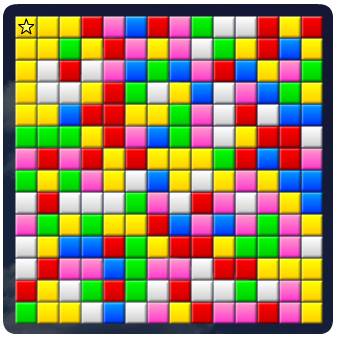
\includegraphics[scale=0.88]{initialState.png}
\end{figure}

\begin{figure}[h!]
  \caption{Estado inicial.}
  \label{regla}
  \centering
    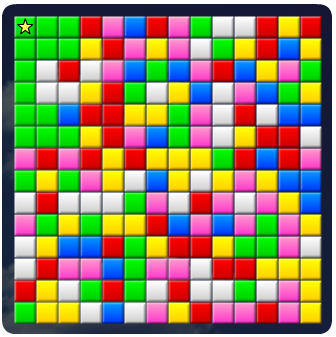
\includegraphics[scale=0.88]{greenRule.png}
\end{figure}

\begin{figure}[h!]
  \caption{Prueba de que h1 no es admisible}
  \label{h1}
  \centering
    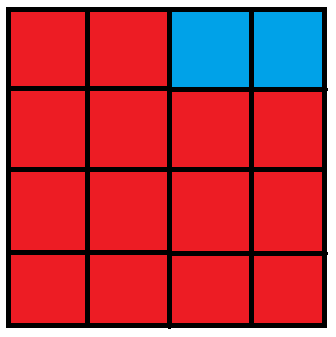
\includegraphics[scale=0.88]{h1.png}
\end{figure}

\begin{figure}[h!]
  \caption{Prueba de que h2 no es admisible}
  \label{h2}
  \centering
    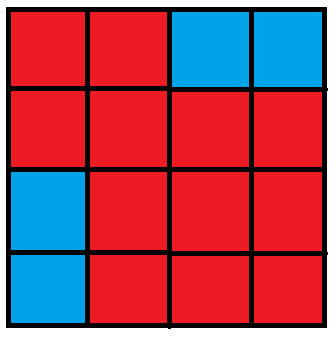
\includegraphics[scale=0.88]{h2.png}
\end{figure}

\begin{figure}[h!]
  \caption{Un tablero gen\'erico}
  \label{mapa}
  \centering
    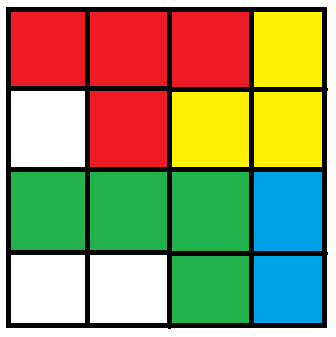
\includegraphics[scale=0.88]{boardToGraph.png}
\end{figure}

\begin{figure}[h!]
  \caption{Grafo que representa el tablero de la figura \ref{mapa}}
  \label{grafo}
  \centering
    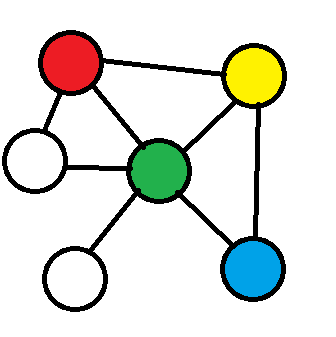
\includegraphics[scale=0.88]{graph.png}
\end{figure}



\begin{table}
  \begin{tabular}{|c|c|c|c|}
  
  \hline
  H1 & H2 & H4 & H3 \\
  \hline
T:432 N:164 & T:220 N:147 & T:211 N:125 & T:1247 N:171 \\
\hline
T:233 N:145 & T:263 N:156 & T:353 N:680 & T:1993 N:218 \\
\hline
T:114 N:100 & T:132 N:135 & T:142 N:135 & T:677 N:163 \\
\hline
T:228 N:145 & T:290 N:420 & T:293 N:145 & T:1455 N:168 \\
\hline
T:482 N:1615 & T:254 N:147 & T:264 N:165 & T:1282 N:167 \\
\hline
  \end{tabular}
  \centering
  \caption{Tabla de que mide tiempos y nodos explotados en un tablero de 14x14 con 30 movimientos m\'aximos. T indica el tiempo en milisegundos y N la cantidad de nodos explotados. Se muestran los resultados para 5 tableros}
  \label{tablaHeuristicas}
\end{table}

\begin{table}
  \begin{tabular}{|c|c|c|c|c|}
\hline
& H1 & H2 & H4 & H3 \\
\hline
WINS & 3 & 1 & 1 & 0 \\
\hline
TIME AVG & 297.8 & 231.8 & 252.6 & 1330.8 \\
\hline
NODE AVG & 433.8 & 201.0 & 250.0 & 177.4 \\  
\hline
\end{tabular}
\centering
	\caption{Tabla que muestra los promedios y cantidad de victorias (en tiempo) de la tabla \ref{tablaHeuristicas}}
    \label{promedios1}
  
\end{table}


\begin{table}
  \begin{tabular}{|c|c|c|c|}
  \hline
  H1 & H2 & H4 & H3 \\
  \hline
DOMINATED & ISLANDS & CORNERS & GRAPH \\
\hline
T:343 N:164 & T:88484 N:35156 & T:198 N:125 & T:1242 N:171 \\
\hline
T:233 N:141 & T:313 N:629 & T:4567 N:9536 & T:1997 N:218 \\
\hline
T:104 N:100 & T:138 N:135 & T:143 N:135 & T:672 N:163 \\
\hline
T:230 N:137 & T:43352 N:23634 & T:398 N:1089 & T:1472 N:168 \\
\hline
T:15335 N:14867 & T:937 N:3471 & T:260 N:151 & T:1277 N:167 \\
\hline
  \end{tabular}
  \centering
  \caption{Tabla de que mide tiempos y nodos explotados en un tablero de 14x14 con 28 movimientos m\'aximos. T indica el tiempo en milisegundos y N la cantidad de nodos explotados. Se muestran los resultados para 5 tableros.}
  \label{tablaHeuristicas2}
\end{table}

\begin{table}
  \begin{tabular}{|c|c|c|c|c|}
\hline
& H1 & H2 & H4 & H3 \\
\hline
WINS & 3 & 0 & 2 & 0 \\
TIME AVG & 3249.0 & 26644.8 & 1113.2 & 1332.0 \\
NODE AVG & 3081.8 & 12605.0 & 2207.2 & 177.4 \\\hline
\end{tabular}
\centering
	\caption{Tabla que muestra los promedios y cantidad de victorias (en tiempo) de la tabla \ref{tablaHeuristicas2}. Notar como la \'unica heur\'istica que mantiene estabilidad con respecto a la tabla \ref{promedios1} es H3. }
  
\end{table}

\begin{table}
  \begin{tabular}{|c|c|c|c|}
  \hline
  H1 & H2 & H4 & H3 \\
  \hline
T:323 N:1181 & T:124 N:1531 & T:15 N:181 & T:153 N:859 \\
\hline
T:34 N:800 & T:10 N:287 & T:138 N:2036 & T:41 N:257 \\
\hline
T:42 N:926 & T:54 N:1112 & T:5 N:118 & T:59 N:572 \\
\hline
T:14 N:293 & T:211 N:2570 & T:6137 N:17211 & T:67 N:660 \\
\hline
 BFS & DFS & ID & \\
 \hline
 T:40043 N:28244 & T:27 N:669 & T:418 N:45606 &\\
 \hline
 T:568 N:4421 & T:50 N:1286 & T:220 N:7929 &\\
 \hline
 T:63090 N:34398 & T:920 N:7007 & T:39169 N:44479 & \\
 \hline
 T:12805 N:18718 & T:6240 N:17575 & T:14921 N:38456 & \\
 \hline
  \end{tabular}
  \caption{Tabla de que mide tiempos y nodos explotados en un tablero de 6x6 con 10 movimientos m\'aximos. T indica el tiempo en milisegundos y N la cantidad de nodos explotados. Se muestran los resultados para 4 tableros.}
  \label{tablaHeuristicas3}
  \centering
\end{table}

\begin{table}
  \begin{tabular}{|c|c|c|c|c|c|c|c|}
\hline
& H1 & H2 & H4 & H3 & BFS & DFS & ID \\
\hline
WINS & 1 & 1 & 2 & 0 & 0 & 0 & 0 \\
\hline
TIME AVG &  103.25 & 99.75 & 1573.75 & 80.0 & 29126.5 & 1809.25 & 13682.0 \\
\hline
NODE AVG & 800.0 & 1375.0 & 4886.5 & 587.0 & 21445.25 & 1809.25 & 13682.0 \\
\hline
\end{tabular}
\centering
	\caption{Tabla que muestra los promedios y cantidad de victorias (en tiempo) de la tabla \ref{tablaHeuristicas3}. Notar como las b\'usquedas informadas son claramente m\'as r\'apidas que las no informadas. }
  
\end{table}
















\end{document}
